%
% $RCSfile: knowledge_representation.tex,v $
%
% Copyright (C) 2002-2008. Christian Heller.
%
% Permission is granted to copy, distribute and/or modify this document
% under the terms of the GNU Free Documentation License, Version 1.1 or
% any later version published by the Free Software Foundation; with no
% Invariant Sections, with no Front-Cover Texts and with no Back-Cover
% Texts. A copy of the license is included in the section entitled
% "GNU Free Documentation License".
%
% http://www.cybop.net
% - Cybernetics Oriented Programming -
%
% http://www.resmedicinae.org
% - Information in Medicine -
%
% Version: $Revision: 1.1 $ $Date: 2008-08-19 20:41:07 $ $Author: christian $
% Authors: Christian Heller <christian.heller@tuxtax.de>
%

\section{Knowledge Representation}
\label{knowledge_representation_heading}
\index{Knowledge Representation}

Section \ref{human_thinking_heading} identified the abstraction principles of
human thinking, before section \ref{design_reflections_heading} reflected on
their impact on software design. The final considerations of this chapter now
deal with a possible architecture for knowledge representation (as first
presented in \cite{heller2006}), which applies the principles of human thinking.

%
% $RCSfile: knowledge_ontology.tex,v $
%
% Copyright (C) 2002-2008. Christian Heller.
%
% Permission is granted to copy, distribute and/or modify this document
% under the terms of the GNU Free Documentation License, Version 1.1 or
% any later version published by the Free Software Foundation; with no
% Invariant Sections, with no Front-Cover Texts and with no Back-Cover
% Texts. A copy of the license is included in the section entitled
% "GNU Free Documentation License".
%
% http://www.cybop.net
% - Cybernetics Oriented Programming -
%
% http://www.resmedicinae.org
% - Information in Medicine -
%
% Version: $Revision: 1.1 $ $Date: 2008-08-19 20:41:07 $ $Author: christian $
% Authors: Christian Heller <christian.heller@tuxtax.de>
%

\subsection{Knowledge Ontology}
\label{knowledge_ontology_heading}
\index{Knowledge Ontology}
\index{Composition}
\index{Ontology}
\index{Ontological Level}
\index{Granularity}

The previous sections tried to demonstrate the importance of \emph{Composition}
for knowledge modelling. One technique that was mentioned in this context are
\emph{Ontologies}. Section \ref{conceptual_network_heading} introduced some of
its numerous definitions. Section \ref{association_elimination_heading}
demonstrated how the principle of \emph{Hierarchy} may be applied to obtain an
\emph{Ontology}. The layers forming an ontology were called
\emph{Ontological Level}.

Basically, an ontology represents a systematic description of complex domain
contexts. This work uses its own adapted definition, and considers an ontology
to be \emph{a strict hierarchy of abstract models, organised in levels of
growing granularity, that are solely unidirectionally related}.

Terminologies as described in section \ref{terminology_heading} may be used to
specify the basic elements of an ontology. Every term may be represented by an
own abstract model (concept) containing a number of strings, one for each
terminology system. Further strings may stand for language translations, which
has importance for \emph{Internationalisation}.

The following examples may seem simple, but want to strengthen the hierarchical
thinking of the reader, under consideration of the granularity of models.

%
% $RCSfile: biological_systems.tex,v $
%
% Copyright (C) 2002-2008. Christian Heller.
%
% Permission is granted to copy, distribute and/or modify this document
% under the terms of the GNU Free Documentation License, Version 1.1 or
% any later version published by the Free Software Foundation; with no
% Invariant Sections, with no Front-Cover Texts and with no Back-Cover
% Texts. A copy of the license is included in the section entitled
% "GNU Free Documentation License".
%
% http://www.cybop.net
% - Cybernetics Oriented Programming -
%
% http://www.resmedicinae.org
% - Information in Medicine -
%
% Version: $Revision: 1.1 $ $Date: 2008-08-19 20:41:05 $ $Author: christian $
% Authors: Christian Heller <christian.heller@tuxtax.de>
%

\subsubsection{Biological Systems}
\label{biological_systems_heading}
\index{Biological System as Ontology}
\index{Ontological Layer}
\index{Parallel Layer}
\index{Stratum}

One example showing the hierarchical structuring of biological systems is
mentioned in \cite{sengbusch}. Its models are listed in decreasing granularity,
in table \ref{biological_table}.

\begin{table}[ht]
    \begin{center}
        \begin{footnotesize}
        \begin{tabular}{| p{105mm} |}
            \hline
            \textbf{Biological System}\\
            \hline
            Ecosystem\\
            \hline
            Biocoenosis (Living Community)\\
            \hline
            Multiple Cell Organism\\
            \hline
            Single Cell Organism (Protozoa)\\
            \hline
            Organelle (Mitochondrie, Chloroplast)\\
            \hline
            Supra Molecular Complex (Ribosome, Chromosome, Membrane)\\
            \hline
            Small Molecule\\
            \hline
        \end{tabular}
        \end{footnotesize}
        \caption{Hierarchical Structuring of Biological Systems}
        \label{biological_table}
    \end{center}
\end{table}

It is important not to mix ontological layers with parallel layers. In
\emph{Geology} or \emph{Biology}, the latter (also called \emph{Stratum}) may
be layers of material arranged one on top of another (such as a layer of tissue
or cells in an organism) \cite{wordnet}. However, these are not \emph{composed}
of each other. Ontological layers, on the other hand, have a different level of
granularity, each so that higher-level abstractions are composed of lower-level
abstractions.

%
% $RCSfile: logical_book.tex,v $
%
% Copyright (C) 2002-2008. Christian Heller.
%
% Permission is granted to copy, distribute and/or modify this document
% under the terms of the GNU Free Documentation License, Version 1.1 or
% any later version published by the Free Software Foundation; with no
% Invariant Sections, with no Front-Cover Texts and with no Back-Cover
% Texts. A copy of the license is included in the section entitled
% "GNU Free Documentation License".
%
% http://www.cybop.net
% - Cybernetics Oriented Programming -
%
% http://www.resmedicinae.org
% - Information in Medicine -
%
% Version: $Revision: 1.1 $ $Date: 2008-08-19 20:41:07 $ $Author: christian $
% Authors: Christian Heller <christian.heller@tuxtax.de>
%

\subsubsection{Logical Book}
\label{logical_book_heading}
\index{Logical Book as Ontology}
\index{Extension of Ontologies}
\index{Physical Book as Ontology}

The logical structure of a \emph{Book} shall serve as second example. A
\emph{Chapter} may consist of \emph{Paragraphs}. Yet it may become necessary to
first subdivide \emph{Chapter} into \emph{Sections} which then consist of
\emph{Paragraphs}, as shown in table \ref{book_table}.

All ontologies can get extended \emph{up-} or \emph{downwards}, by adding
further levels, at any later point in design time. But they can as well get
extended by inserting \emph{Intermediate Layers} between two already existing
ones. However, additional levels should only get introduced if there really is
a need for them.

\begin{table}[ht]
    \begin{center}
        \begin{footnotesize}
        \begin{tabular}{| p{105mm} |}
            \hline
            \textbf{Model Category}\\
            \hline
            Library\\
            \hline
            Book\\
            \hline
            Part\\
            \hline
            Chapter\\
            \hline
            Section\\
            \hline
            Paragraph\\
            \hline
            Sentence\\
            \hline
            Word\\
            \hline
            Character\\
            \hline
        \end{tabular}
        \end{footnotesize}
        \caption{Logical Book}
        \label{book_table}
    \end{center}
\end{table}

In contrast to the division of a \emph{logical} book, a \emph{physical} book
may be structured completely differently, for example into \emph{Binding},
\emph{Cover} and \emph{Pages}. Of course, the contents of an ontology heavily
depends on the intended area of application (knowledge domain) of the software
to be created.

%
% $RCSfile: interdisciplinary_science.tex,v $
%
% Copyright (C) 2002-2008. Christian Heller.
%
% Permission is granted to copy, distribute and/or modify this document
% under the terms of the GNU Free Documentation License, Version 1.1 or
% any later version published by the Free Software Foundation; with no
% Invariant Sections, with no Front-Cover Texts and with no Back-Cover
% Texts. A copy of the license is included in the section entitled
% "GNU Free Documentation License".
%
% http://www.cybop.net
% - Cybernetics Oriented Programming -
%
% http://www.resmedicinae.org
% - Information in Medicine -
%
% Version: $Revision: 1.1 $ $Date: 2008-08-19 20:41:07 $ $Author: christian $
% Authors: Christian Heller <christian.heller@tuxtax.de>
%

\subsubsection{Interdisciplinary Science}
\label{interdisciplinary_science_heading}
\index{Interdisciplinary Science}
\index{System of Sciences}
\index{Sciences as Ontology}
\index{Cybernetics}

A third, certainly very subjective example tries to sort a number of known
\emph{Sciences} into one common system (table \ref{sciences_table}).
\emph{Arts}, \emph{Linguistics}, \emph{Mathematics} and \emph{Informatics} have
an extra status: They deal with already abstracted knowledge (paintings, music,
language, numbers) and can be used as utility by any of the other sciences.

\begin{table}[ht]
    \begin{center}
        \begin{footnotesize}
        \begin{tabular}{| p{35mm} | p{70mm} |}
            \hline
            \textbf{Scientific Subject} & \textbf{Example Model}\\
            \hline
            Astronomy & Celestial Body (Big Bang, Cosmos)\\
            \hline
            Biology & Living Thing (Human, Animal, Plant, Virus)\\
            \hline
            Geography & Dead Thing (Air, Fire, Stone, Crystal)\\
            \hline
            Chemistry & Compounds (Water, DNA)\\
            \hline
            Physics & Particles (Elementary Particle, Atom, Matter, Energy)\\
            \hline
            Philosophy / Religion & Dialectic Dualism (Matter/Anti-Matter, +/-, 0/1)\\
            \hline
        \end{tabular}
        \end{footnotesize}
        \caption{System of Sciences}
        \label{sciences_table}
    \end{center}
\end{table}

The whole effort of finding new ways for representing knowledge, as done in
this work, is an \emph{inter-disciplinary} undertaking itself, touching various
fields of science. The world (nature) needs to be understood in its basics so
that humans are enabled to copy its concepts and put them into artificial
models -- exactly what \emph{Cybernetics} is all about.

%
% $RCSfile: car_model.tex,v $
%
% Copyright (C) 2002-2008. Christian Heller.
%
% Permission is granted to copy, distribute and/or modify this document
% under the terms of the GNU Free Documentation License, Version 1.1 or
% any later version published by the Free Software Foundation; with no
% Invariant Sections, with no Front-Cover Texts and with no Back-Cover
% Texts. A copy of the license is included in the section entitled
% "GNU Free Documentation License".
%
% http://www.cybop.net
% - Cybernetics Oriented Programming -
%
% http://www.resmedicinae.org
% - Information in Medicine -
%
% Version: $Revision: 1.1 $ $Date: 2008-08-19 20:41:05 $ $Author: christian $
% Authors: Christian Heller <christian.heller@tuxtax.de>
%

\subsubsection{Car Model}
\label{car_model_heading}
\index{Car Model as Ontology}
\index{Computer Aided Design}
\index{CAD}
\index{Computer Aided Manufacturing}
\index{CAM}
\index{Unidirectional Relation}
\index{Layers of an Abstract Model}
\index{Levels of an Abstract Model}

A \emph{Computer Aided Design} (CAD)/ \emph{Computer Aided Manufacturing} (CAM)
system of a car manufacturer will have a \emph{Car} model like the one shown in
table \ref{car_table}.

\begin{table}[ht]
    \begin{center}
        \begin{footnotesize}
        \begin{tabular}{| p{105mm} |}
            \hline
            \textbf{Model Category}\\
            \hline
            Car\\
            \hline
            Body, Chassis, Engine, Transmission\\
            \hline
            Door, Axle, Wheel, Cylinder\\
            \hline
            Window, Suspension, Plunger\\
            \hline
        \end{tabular}
        \end{footnotesize}
        \caption{Car Model}
        \label{car_table}
    \end{center}
\end{table}

The ontology contains multiple categories of models which are composed of each
other. An \emph{Engine} consists of a \emph{Cylinder} which consists of a
\emph{Plunger} and so on. That is why people speak of different \emph{Layers}
or \emph{Levels} of abstract models. An \emph{Axle} belongs to one level and a
\emph{Chassis} belongs to another, higher level. In a good ontology, the
relations between models are always \emph{unidirectional}, that is a chassis
can link to axles but not the other way.

%
% $RCSfile: macrocosm_and_microcosm.tex,v $
%
% Copyright (C) 2002-2008. Christian Heller.
%
% Permission is granted to copy, distribute and/or modify this document
% under the terms of the GNU Free Documentation License, Version 1.1 or
% any later version published by the Free Software Foundation; with no
% Invariant Sections, with no Front-Cover Texts and with no Back-Cover
% Texts. A copy of the license is included in the section entitled
% "GNU Free Documentation License".
%
% http://www.cybop.net
% - Cybernetics Oriented Programming -
%
% http://www.resmedicinae.org
% - Information in Medicine -
%
% Version: $Revision: 1.1 $ $Date: 2008-08-19 20:41:07 $ $Author: christian $
% Authors: Christian Heller <christian.heller@tuxtax.de>
%

\subsubsection{Macrocosm and Microcosm}
\label{macrocosm_and_microcosm_heading}
\index{Macrocosm as Part of an Ontology}
\index{Microcosm as Part of an Ontology}
\index{Astronomical Particles as Ontology}
\index{Universe}
\index{Top Level Model}
\index{Concept}
\index{Electronic Health Record}
\index{EHR}
\index{Electronic Insurance Record}
\index{EIR}

Table \ref{astronomical_table} lists \emph{Astronomical Particles}
\cite{fernandezdavid, arnett}. It ends with the \emph{Universe} and an
undefinable \emph{Macrocosm}.

\begin{table}[ht]
    \begin{center}
        \begin{footnotesize}
        \begin{tabular}{| p{40mm} | p{65mm} |}
            \hline
            \textbf{Category} & \textbf{Example Model}\\
            \hline
            Macrocosm & (Infinity)\\
            \hline
            Universe & Our Universe with its Laws of Nature\\
            \hline
            Heap of Galaxies & Local Group, Heap of Virgo\\
            \hline
            Galaxy & Milky Way (our), Andromeda, Magellan's Clouds\\
            \hline
            Planetary (Solar) System & Sol (Sun), 51 Pegasi\\
            \hline
            Star/ Planet & Beta Pictoris, Mercury, Venus, Earth, Mars\\
            \hline
        \end{tabular}
        \end{footnotesize}
        \caption{Astronomical Particles}
        \label{astronomical_table}
    \end{center}
\end{table}

When trying to abstract things (in software), there has to be some limit, a
kind of \emph{Top Level Model}. It represents the \emph{Concept} to be
described. For a medical information system, one such top level model will be
the \emph{Electronic Health Record} (EHR); for an insurance application, it
will be the \emph{Electronic Insurance Record} (EIR); and so on.

Models do not only have to be limited \emph{upwards}; the same holds true for
modelling towards \emph{Microcosm}. Table \ref{physical_table} organises
particles, as used by natural sciences, into several categories.

\begin{table}[ht]
    \begin{center}
        \begin{footnotesize}
        \begin{tabular}{| p{50mm} | p{55mm} |}
            \hline
            \textbf{Category} & \textbf{Example Model}\\
            \hline
            Physical Compound & Air, Water, Fire, Ground\\
            \hline
            Chemical Compound/ Molecule & H$_{2}$, O$_{2}$, O$_{3}$, H$_{2}$O\\
            \hline
            Crystal & C (Diamond)\\
            \hline
            Atom (Chemical Element) & H, He, O\\
            \hline
            Elementary Particle & Quark, Lepton (Electron, Neutrino)\\
            \hline
            Urelement & (Primary Particle)\\
            \hline
            Microcosm & (Infinity)\\
            \hline
        \end{tabular}
        \end{footnotesize}
        \caption{Physical Particles}
        \label{physical_table}
    \end{center}
\end{table}

Although the real world seems to be built like that (infinite, nobody knowing
what comes beneath the \emph{Quark} particles) -- in software modelling it
makes no sense (and is actually impossible) to neverendingly introduce lower
and lower levels, towards \emph{Microcosm}. On some point, the hierarchy has to
be stopped, to be able to abstract it in software. The later chapter
\ref{state_and_logic_heading} gives an overview of common knowledge primitives.


%
% $RCSfile: schema.tex,v $
%
% Copyright (C) 2002-2008. Christian Heller.
%
% Permission is granted to copy, distribute and/or modify this document
% under the terms of the GNU Free Documentation License, Version 1.1 or
% any later version published by the Free Software Foundation; with no
% Invariant Sections, with no Front-Cover Texts and with no Back-Cover
% Texts. A copy of the license is included in the section entitled
% "GNU Free Documentation License".
%
% http://www.cybop.net
% - Cybernetics Oriented Programming -
%
% http://www.resmedicinae.org
% - Information in Medicine -
%
% Version: $Revision: 1.1 $ $Date: 2008-08-19 20:41:08 $ $Author: christian $
% Authors: Christian Heller <christian.heller@tuxtax.de>
%

\subsection{Schema}
\label{schema_heading}
\index{Schema with Meta Information}
\index{Knowledge Schema with Meta Information}
\index{Model}
\index{Concept}
\index{Item}
\index{Category}
\index{Compound}
\index{Discrimination}
\index{Categorisation}
\index{Composition}
\index{Compound Model}
\index{Meta Information}
\index{Meta Model}

A theoretical \emph{Model} is an abstract clip of the real world, and exists in
the human mind. Another common word for \emph{Model} is \emph{Concept}. It is
the subsumption of \emph{Item}, \emph{Category} and \emph{Compound}, resulting
from three activities of abstraction: \emph{Discrimination}, \emph{Categorisation}
and \emph{Composition} (section \ref{abstraction_heading}). As such, each model
\emph{knows} about the parts it consists of.

\begin{figure}[ht]
    \begin{center}
        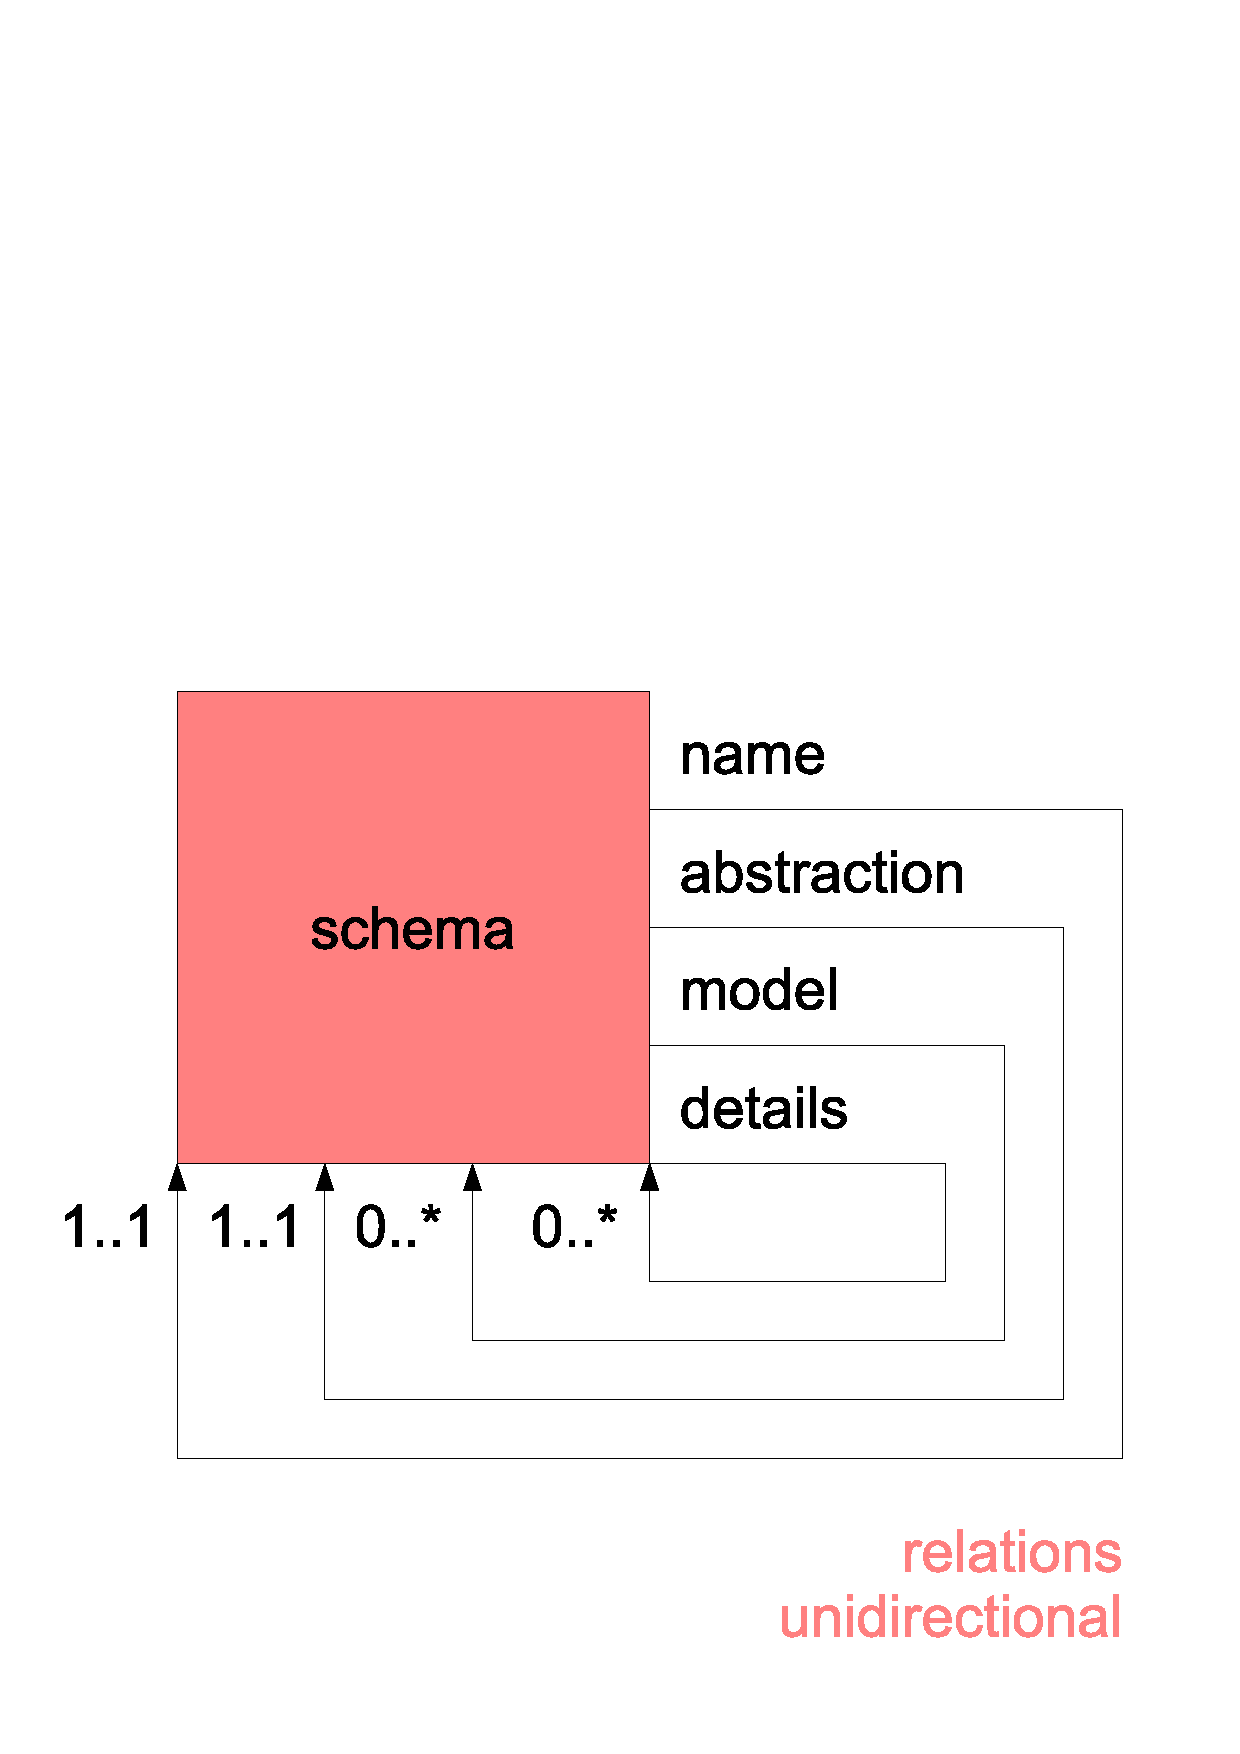
\includegraphics[scale=0.3,angle=-90]{graphic/schema.pdf}
        \caption{Knowledge Schema with Meta Information about Parts}
        \label{schema_figure}
    \end{center}
\end{figure}

Yet what does this knowledge of a compound model (whole) about its parts imply?
Software developers call knowledge \emph{about} something \emph{Meta Information}.
Figure \ref{schema_figure} shows the four essential kinds of meta information in
a whole-part relation. Software developers might want to call the illustration
of these relations a \emph{Schema} or \emph{Meta Model}.

An obvious way is to give each part a unique \emph{Name} for identification.
The concept of a human body, for example, would have parts like heart, brain,
left\_arm and so on.

Secondly, a compound needs to know about the \emph{Model} of each part since a
part may itself be seen as compound that needs to know about its parts. Although
all real world items can be modelled as compound, it does not make sense to do
so in the virtual world of the human mind. As mentioned before, models have to
be limited in their information contents, towards microcosm as well as towards
macrocosm, in order to be comprehensible by the human mind. It is therefore
necessary to introduce primitive models like a word or a number (compare
\emph{Quality and Quantity}, section \ref{quality_and_quantity_heading}),
representing the final form of abstraction in a compound.

The distinction of the several kinds of models, in other words the kind of
\emph{Abstraction} (compound, term, number etc.) of a model is the third
kind of information a compound needs to know about its parts. It is comparable
to a \emph{Type} in classical system programming languages (section
\ref{system_programming_heading}).

All further kinds of meta information are summed up by a fourth relation which
is called \emph{Details} in this work. Just like the \emph{Model}, it is a
dynamically extensible structure. It will be explained in the following section.

The suggested knowledge model uses a simple \emph{Tree} structure, capable of
referencing parts of arbitrary type. It does not follow the \emph{Composite}
software pattern (section \ref{composite_heading}), because the meta information
whether a part model is a compound (composite) or not (leaf) does not belong
into the model structure. Section \ref{categorisation_versus_composition_heading}
explained this design mistake on the example of \emph{Party} types. It is not
good to fix some model as leave, at design time. Who knows if at runtime
(during program execution), that model would not have to have any parts?
As an aside: A similar design (simple tree structure) is used by the
\emph{Java Swing} framework \cite{java}, for example. Its tree node class
\emph{DefaultMutableTreeNode} represents a \emph{Tree Node} and
\emph{Tree Container}, at the same time.

%
% $RCSfile: double_hierarchy.tex,v $
%
% Copyright (C) 2002-2008. Christian Heller.
%
% Permission is granted to copy, distribute and/or modify this document
% under the terms of the GNU Free Documentation License, Version 1.1 or
% any later version published by the Free Software Foundation; with no
% Invariant Sections, with no Front-Cover Texts and with no Back-Cover
% Texts. A copy of the license is included in the section entitled
% "GNU Free Documentation License".
%
% http://www.cybop.net
% - Cybernetics Oriented Programming -
%
% http://www.resmedicinae.org
% - Information in Medicine -
%
% Version: $Revision: 1.1 $ $Date: 2008-08-19 20:41:06 $ $Author: christian $
% Authors: Christian Heller <christian.heller@tuxtax.de>
%

\subsection{Double Hierarchy}
\label{double_hierarchy_heading}
\index{Double Hierarchy}
\index{Whole-Part Relationship}
\index{Dialectical Relationship between Whole and Part}
\index{Conceptual Interaction}
\index{Part}
\index{Property}
\index{Constraint}

Finally, what makes up the character of a model (in the understanding of the
human mind) is a combination of two hierarchies: the \emph{Parts} it consists
of, together with \emph{Meta Information} about it.

Most properties of a molecule in \emph{Chemistry}, for example, are determined
by the number and arrangement of its atoms. \emph{Hydrogen} (H$_{2}$) becomes
\emph{Water} (H$_{2}$O) (with a totally different character) when just one
\emph{Oxygen} (O) atom is added per hydrogen molecule. The Wikipedia Encyclopedia
\cite{wikipedia} cites and writes about Richard Levins and Richard Lewontin
who, in their book \textit{The Dialectical Biologist} \cite{levins}, sketch a
\emph{dialectical} approach to biology:

\begin{quote}
    They focus on the (dialectical) relationship between the \emph{Whole} (or
    \emph{Totality}) and the \emph{Parts}: \textit{Part makes Whole, and Whole
    makes Part} \cite[p. 272]{levins}. That is, a biological system of some kind
    consists of a collection of heterogeneous parts. All of these contribute to
    the character of the whole, as in reductionist thinking. On the other hand,
    the whole has an existence independent of the parts and feeds back to affect
    and determine the nature of the parts. This back-and-forth (dialectic) of
    causation implies a dynamic process. \ldots\ Further, each species is part
    of the \emph{Environment} of all of the others.
\end{quote}

The kinds of meta information discussed in the previous sections were also
called \emph{Dimensions} or \emph{Conceptual Interaction} between a \emph{Whole}
and its \emph{Parts}. They may represent very different properties and each of
them may be constrained to certain values- or areas of validity.

\begin{figure}[ht]
    \begin{center}
        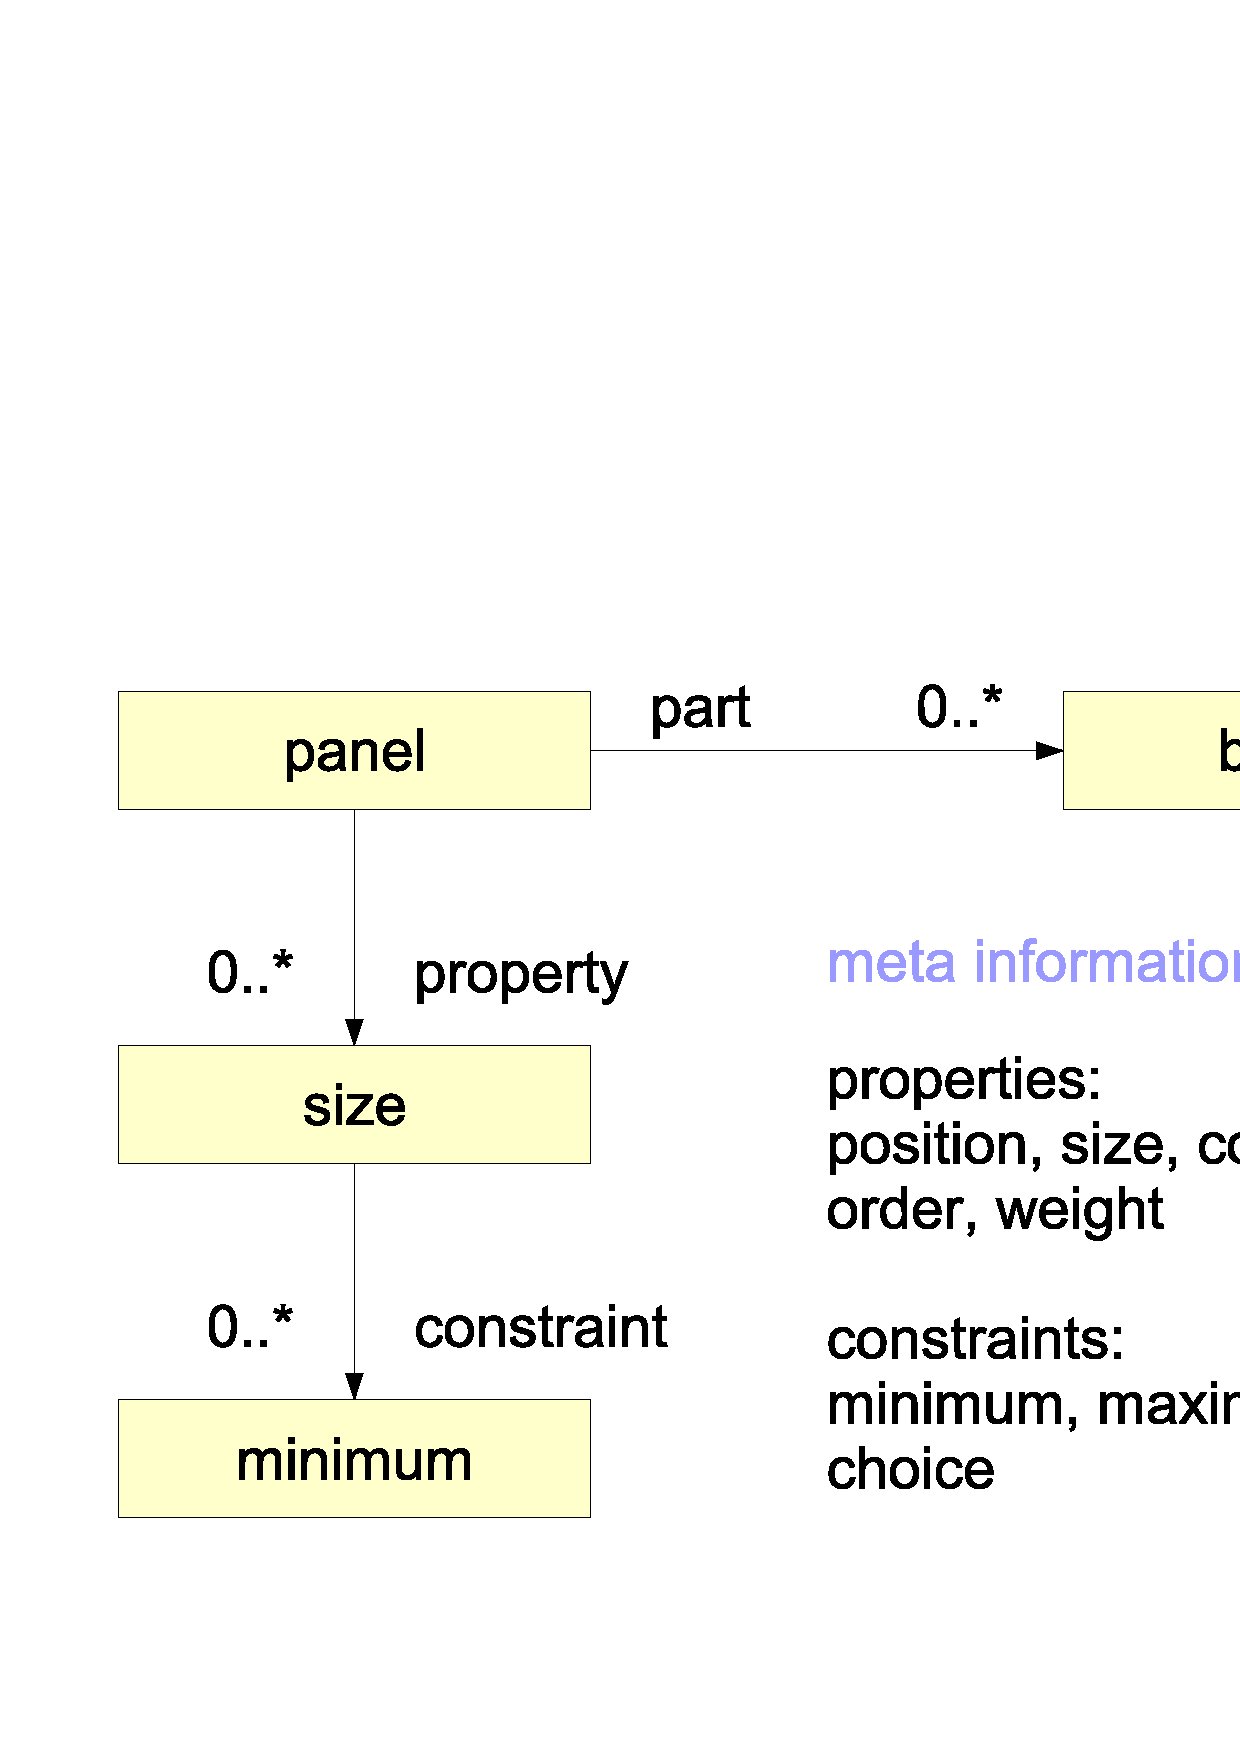
\includegraphics[scale=0.3,angle=-90]{graphic/double.pdf}
        \caption{Double Hierarchy of Parts and Meta Information}
        \label{double_figure}
    \end{center}
\end{figure}

Figure \ref{double_figure} illustrates the \emph{Double Hierarchy} here
spoken of. A graphical panel was chosen as example model. It may consist of
smaller parts, among them being a number of buttons. Altogether, they form the
\emph{Part Hierarchy}. On the other hand, there are properties like the size,
position or colour of the buttons, which are neither part of the panel, nor of
the buttons themselves; they are information \emph{about} the buttons and form
an own \emph{Meta Hierarchy}. To the latter do also belong constraints like the
minimum size of a button or a possible choice of colours for it. Constraints can
be treated like meta information about properties. Once again: \emph{Properties}
are information about a \emph{Part}; \emph{Constraints} are information about a
\emph{Property}.

%
% $RCSfile: modelling_example.tex,v $
%
% Copyright (C) 2002-2008. Christian Heller.
%
% Permission is granted to copy, distribute and/or modify this document
% under the terms of the GNU Free Documentation License, Version 1.1 or
% any later version published by the Free Software Foundation; with no
% Invariant Sections, with no Front-Cover Texts and with no Back-Cover
% Texts. A copy of the license is included in the section entitled
% "GNU Free Documentation License".
%
% http://www.cybop.net
% - Cybernetics Oriented Programming -
%
% http://www.resmedicinae.org
% - Information in Medicine -
%
% Version: $Revision: 1.1 $ $Date: 2008-08-19 20:41:07 $ $Author: christian $
% Authors: Christian Heller <christian.heller@tuxtax.de>
%

\subsection{Modelling Example}
\label{modelling_example_heading}
\index{Modelling Example}
\index{Concept of a Horse}
\index{Structured- and Procedural Programming}
\index{SPP}
\index{Object Oriented Programming}
\index{OOP}
\index{is-a Relation}
\index{has-a Relation}
\index{is-of Relation}
\index{Relation (is-a, has-a, is-of)}

Another example shall be given to substantiate the need to distinguish between
the several kinds of information. How would one describe a \emph{Horse},
unbiassed as a child, by doing some brainstorming? Figure \ref{horse_figure}
shows a number of terms commonly used to create a model of a horse. Most
importantly, there are structural observations describing the horse as concept
consisting of parts like \emph{Head}, \emph{Legs} or \emph{Hoofs}. Secondly,
there are properties like the horse's \emph{Colour}, \emph{Shape} or
\emph{Size}. Thirdly, there are terms describing a horse's actions like its
\emph{Movement} or \emph{Eating}, that change a horse's position and/ or state.
Finally, there are a number of terms like \emph{Hay} or \emph{Saddle}
associating concepts related to the horse.

\begin{figure}[ht]
    \begin{center}
        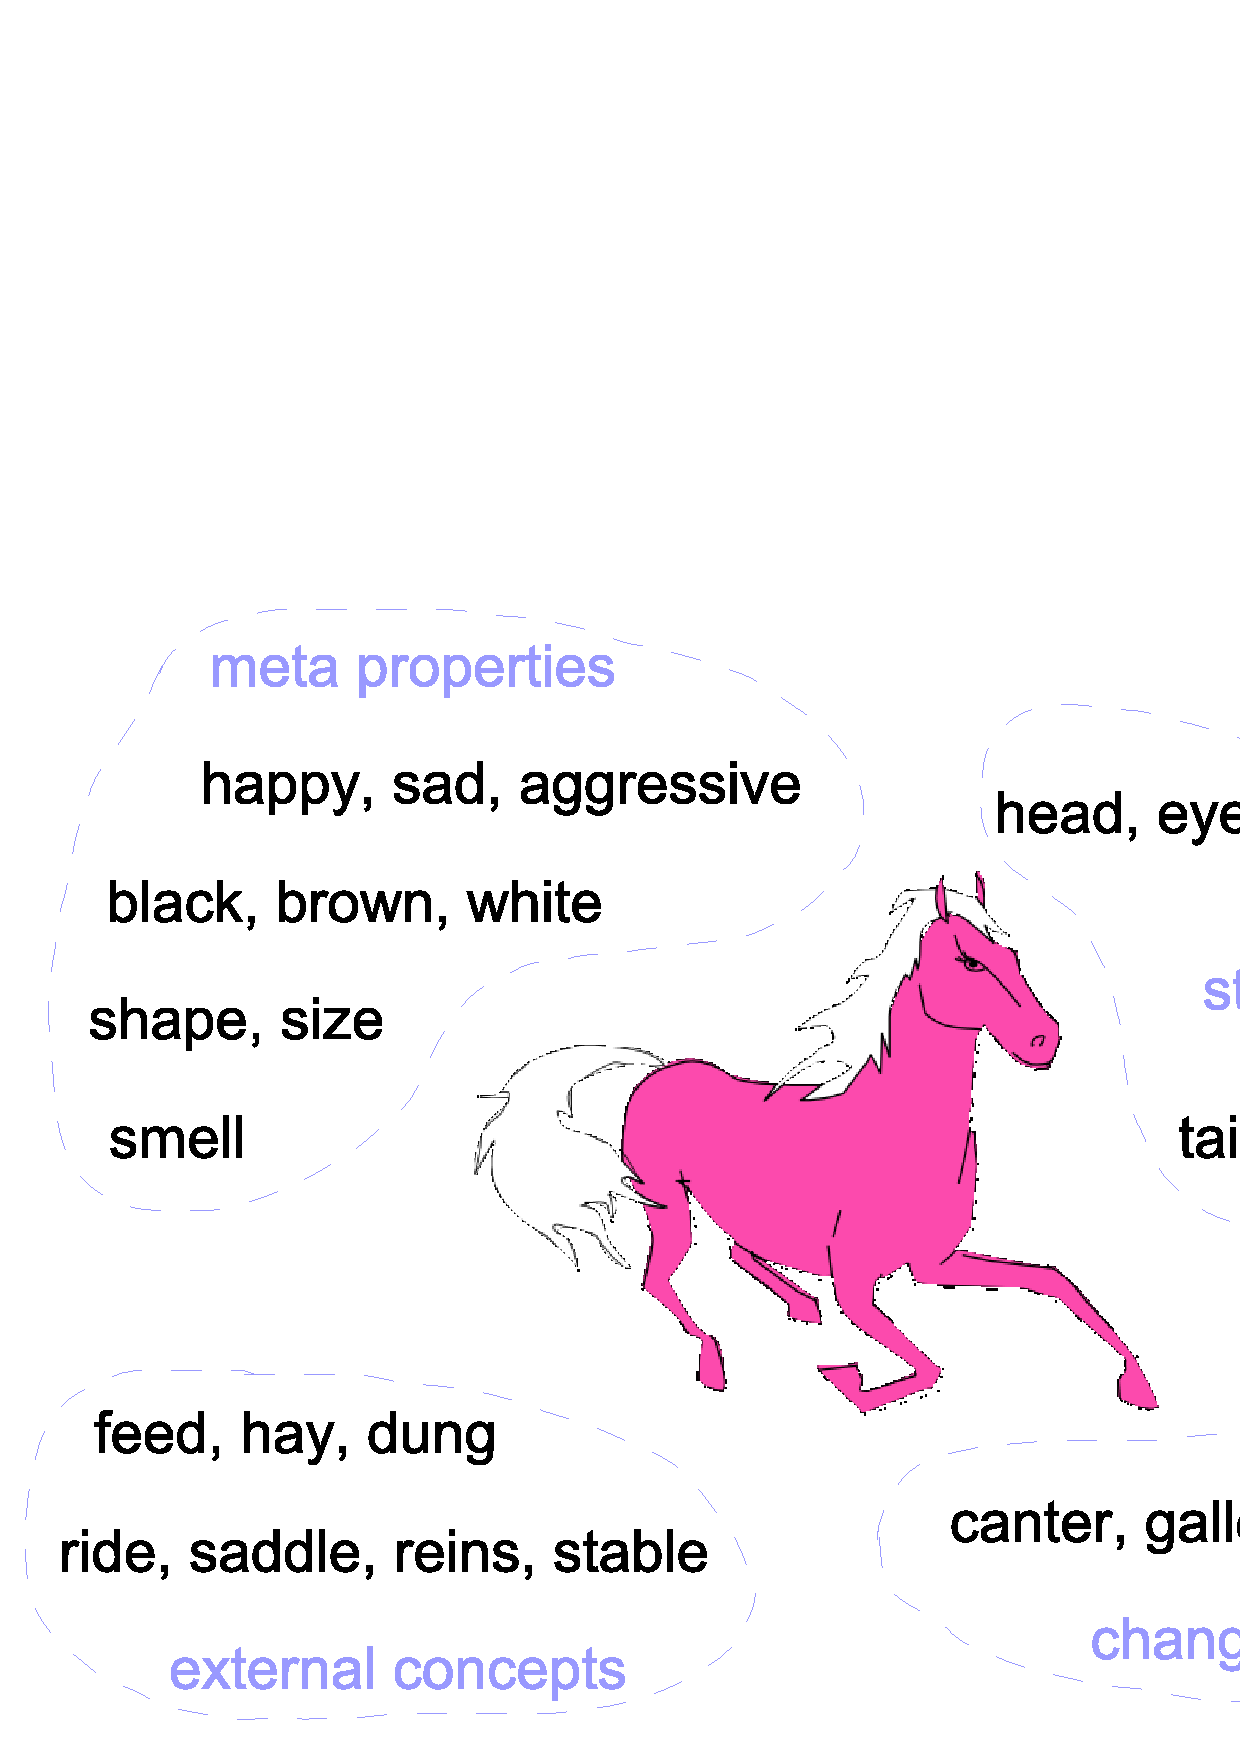
\includegraphics[scale=0.3,angle=-90]{graphic/horse.pdf}
        \caption{Concept of a Horse with Structure, Meta Properties and Logic}
        \label{horse_figure}
    \end{center}
\end{figure}

One might suggest to model properties like the position, size or colour of a
horse's leg as \emph{Part} of that leg. In fact, this is how classical
programming approaches its solutions.
\emph{Structured- and Procedural Programming} (SPP)
(section \ref{structured_and_procedural_programming_heading}), for example,
would probably use a structure called \emph{struct} or \emph{record}
representing the leg and a field standing for the leg's colour. Similarly,
\emph{Object Oriented Programming} (OOP)
(section \ref{object_oriented_programming_heading}) would use a class
representing the leg and an attribute standing for the leg's colour, which, in
Java source code, would look as follows:

\begin{scriptsize}
    \begin{verbatim}
    public class Leg {
        private String knee;
        private String hoof;
        private String colour;
    }
    \end{verbatim}
\end{scriptsize}

However, when following the modelling principles of human thinking (section
\ref{human_thinking_heading}), this is \emph{not} correct! It is true that in
everyday language, one tends to say \textit{A horse leg \emph{has a} colour.}
Unfortunately, this leads to the wrong assumption that a leg were made of a
colour. But this is not the case. A leg does not \emph{consist} of a colour in
the hierarchical meaning of a whole consisting of parts. The colour is rather
property information \emph{about} the leg. It seems there is no correct
expression in natural (English) language stating the property of something. The
\emph{IS-A} verbalisation is used to express that the leg belongs to a special
category of items, for example: \textit{A leg is a body element.} The
\emph{HAS-A} formulation is used to express that a leg as whole consists of
smaller parts, for example: \textit{A leg has a knee and it has a hoof.} But
which formulation expresses a property? Well, perhaps it would be best to say:
\textit{A leg IS-OF a colour.}

It seems that scientists (including the author of this work) and adults in
general have unlearnt to think simple like children. Scientists sometimes tend
to unnecessarily complicate things that can be described quite easy. Other
times, they simplify things which better be distinguished. And looking back
into the history of programming, one wonders who ever had this idea of mixing
structural elements, properties with meta information and logic algorithms into
just one structural entity as at least SPP (record, struct) and OOP (class) do.

The CYBOP knowledge schema introduced before takes care of these things and
distinguishes whole-part- from meta information. Actions (like the gallop of a
horse) causing some change in the model (horse) or its environment are called
\emph{Logic} in this work, since they follow certain rules. Chapter
\ref{state_and_logic_heading} will deal with these.

%
% $RCSfile: container_unification.tex,v $
%
% Copyright (C) 2002-2008. Christian Heller.
%
% Permission is granted to copy, distribute and/or modify this document
% under the terms of the GNU Free Documentation License, Version 1.1 or
% any later version published by the Free Software Foundation; with no
% Invariant Sections, with no Front-Cover Texts and with no Back-Cover
% Texts. A copy of the license is included in the section entitled
% "GNU Free Documentation License".
%
% http://www.cybop.net
% - Cybernetics Oriented Programming -
%
% http://www.resmedicinae.org
% - Information in Medicine -
%
% Version: $Revision: 1.1 $ $Date: 2008-08-19 20:41:06 $ $Author: christian $
% Authors: Christian Heller <christian.heller@tuxtax.de>
%

\subsection{Container Unification}
\label{container_unification_heading}
\index{Container Unification}
\index{Container}
\index{Collection as Container}
\index{Array as Container}
\index{Vector as Container}
\index{Stack as Container}
\index{Set as Container}
\index{List as Container}
\index{Map as Container}
\index{Hash Map as Container}
\index{Hash Table as Container}
\index{Tree as Container}

Section \ref{falsifying_polymorphism_heading} demonstrated how container
inheritance, due to polymorphism, may cause unpredictable behaviour leading to
\emph{falsified} container contents. The sections of this chapter introduced a
knowledge schema which they claimed to be \emph{general}. But that also means
that all kinds of containers must be representable by the suggested schema. But
why are there so many different kinds of containers? What actually is a
container?

It is a concept expressing that some model \emph{contains} some other model(s).
Types of containers that were introduced in section \ref{container_heading} are
\emph{Collections} (Array, Vector, Stack, Set, List), \emph{Maps} (Hash Map,
Hash Table) and the \emph{Tree}. They all are containers. What differs is just
the meta information they store about their elements. A list, for example,
holds position information about each of its elements. A map relates the name
of an element to its model (1:1). A tree links one model to many others (1:n).

But does the different meta information a container holds about its elements
justify the existence of different container models? If a knowledge schema was
general enough to represent a container structure on one hand, and to express
different kinds of meta information on the other, it might be able to behave
like \emph{any} of the known container types.

The schema proposed in this work claims to be this kind of knowledge schema. It
has a container structure by default, and can thus hold many parts in a
\emph{Tree}-like manner. It holds standard meta information about its parts:
their \emph{Name}, \emph{Model}, kind of \emph{Abstraction} and further meta
information called \emph{Details} -- and is therefore able to link the name of
an element to its model, in a \emph{Map}-like manner. To the additional meta
information (details) may belong the \emph{Position} of an element within its
model, in a \emph{List}-like manner. A \emph{Table} structure can be represented
as well, by splitting it into a hierarchical (tree-like) representation, as
known from markup languages (section \ref{markup_language_heading}).

Chapter \ref{cybernetics_oriented_language_heading} will introduce a language
capable of expressing all aspects of the knowledge schema as proposed in this
chapter.

%
% $RCSfile$
%
% Copyright (c) 2002-2006. Christian Heller. All rights reserved.
%
% Permission is granted to copy, distribute and/or modify this document
% under the terms of the GNU Free Documentation License, Version 1.1 or
% any later version published by the Free Software Foundation; with no
% Invariant Sections, with no Front-Cover Texts and with no Back-Cover
% Texts. A copy of the license is included in the section entitled
% "GNU Free Documentation License".
%
% http://www.cybop.net
% - Cybernetics Oriented Programming -
%
% http://www.resmedicinae.org
% - Information in Medicine -
%
% Version: $Revision$ $Date$ $Author$
% Authors: Christian Heller <christian.heller@tuxtax.de>
%

\subsubsection{Universal Memory Structure}
\label{universal_memory_structure_heading}

To better explain the differences between traditional- and cybernetics-oriented
design models, an example shall help. (A first one was given in section
\ref{modelling_mistakes_heading}, which showed modelling mistakes at the
concept of a horse.) Figure \ref{universal_figure} illustrates design-time
structures in the upper half, and runtime structures in the lower. Using
\emph{Structured- and Procedural Programming} (SPP) or
\emph{Object Oriented Programming} (OOP), a developer would design a model as
shown on the upper left-hand side in the figure. (The fact that OOP also offers
inheritance relations and OOP classes do own methods in addition to attributes,
while SPP structures do not, is of minor importance here.) At runtime, exactly
that model would be applied to structure instances and their relations
accordingly, as shown on the lower left-hand side in the figure.

\begin{figure}[ht]
    \begin{center}
        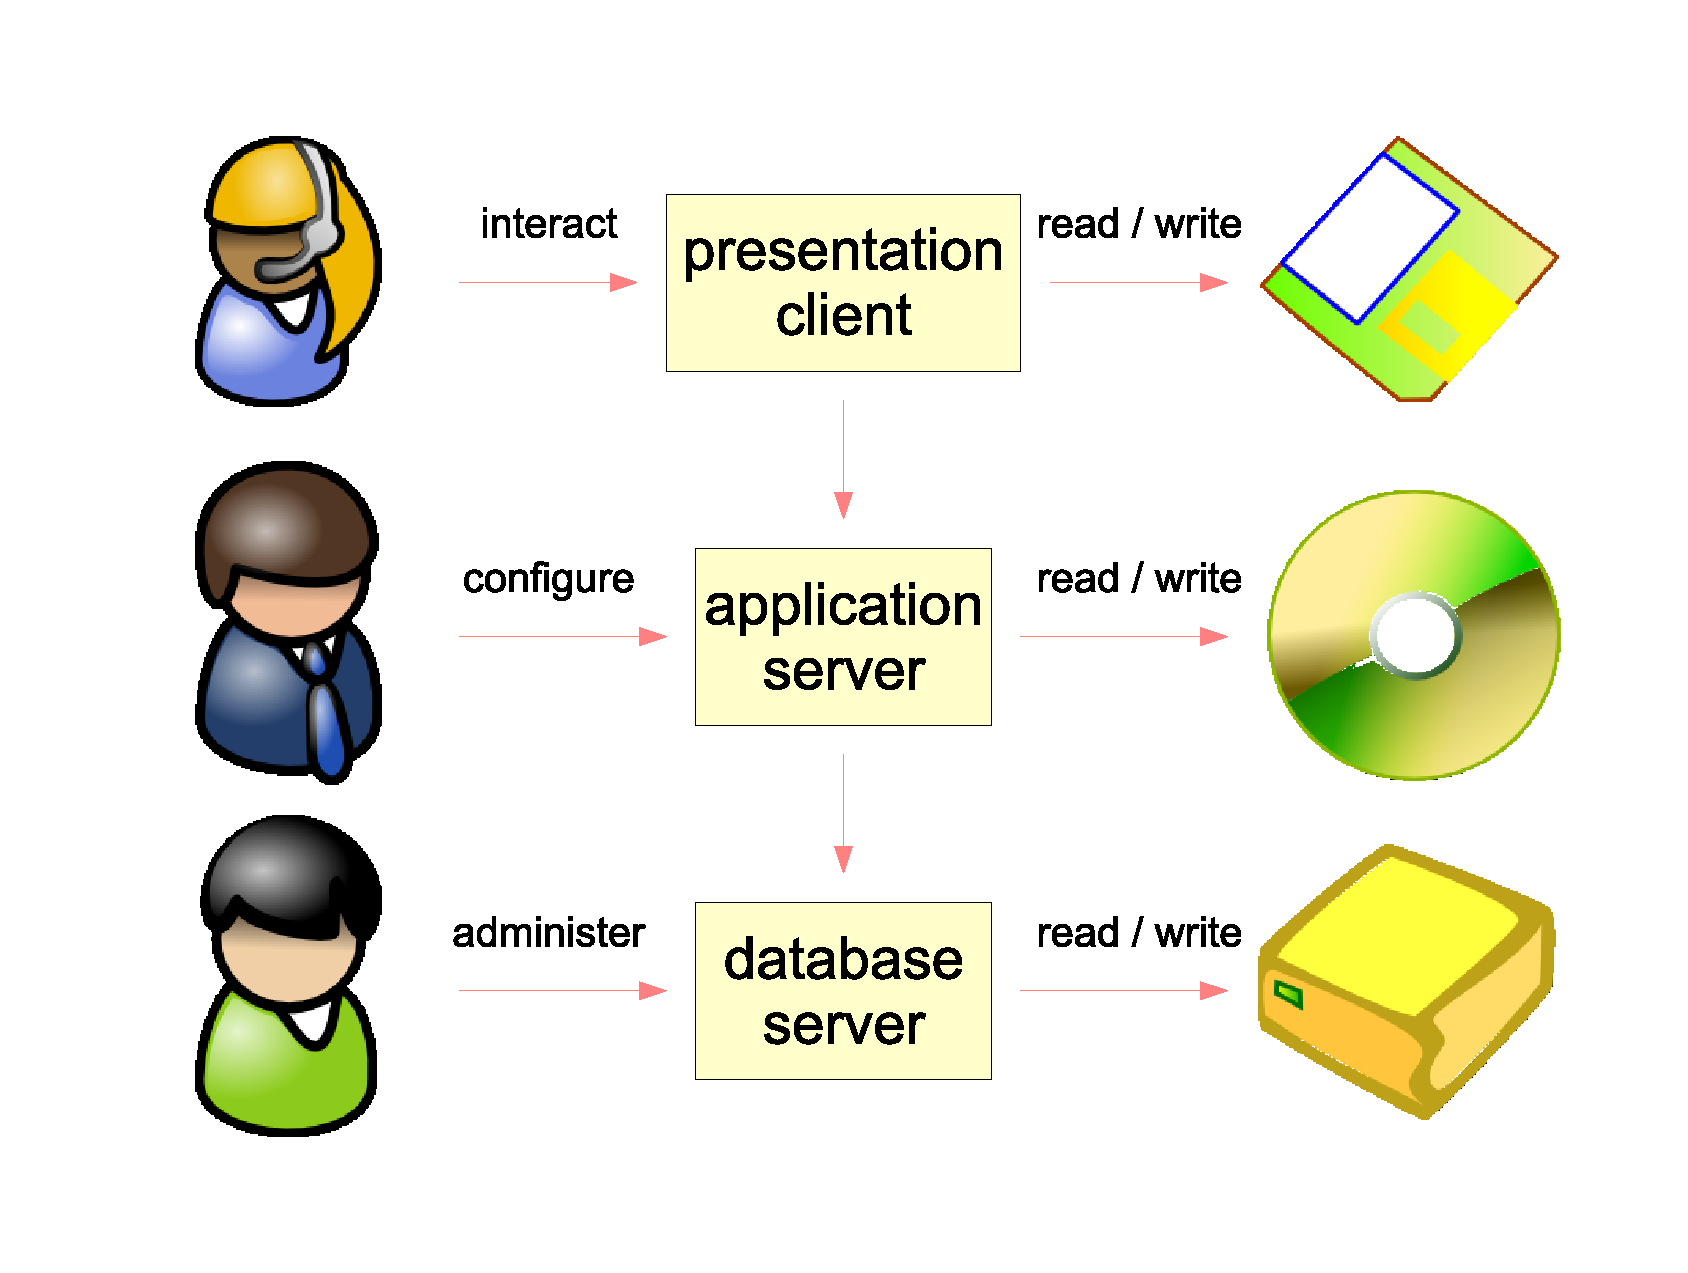
\includegraphics[scale=0.2]{vector/universal.eps}
        \caption{Universal Memory Structure}
        \label{universal_figure}
    \end{center}
\end{figure}

Not so in \emph{Cybernetics Oriented Programming} (CYBOP). Knowledge templates
as created at design time do always have a hierarchical structure, as shown on
the upper right-hand side in the figure. They include \emph{Whole-Part-} as
well as \emph{Meta Hierarchies} (the latter neglected in the figure). At
runtime, these templates get cloned by creating models that follow the
structure of the CYBOP \emph{Knowledge Schema}, as shown on the lower
right-hand side in the figure. While SPP/ OOP rely on a variety of different
structures to store knowledge in memory, CYBOP uses one
\emph{Universal Memory Structure} (knowledge schema) that, so to say, merges
traditional structures like different kinds of \emph{Containers}, \emph{Class}
and \emph{Record}/\emph{Struct}. Even algorithmic structures (logic)
traditionally stored in a \emph{Procedure} are covered by this knowledge
schema. More on state and logic in the following section.

The advantages are obvious. Data available in a unified structure are easier to
process. Dependencies of the knowledge schema are defined clearly and remain
the same for all applications, so that domain/ application knowledge becomes
independent from the underlying system control software. Global data access and
bidirectional dependencies are not necessary anymore, since every knowledge
model can be accessed along well-defined paths within the knowledge hierarchy.
Byte code manipulation and similar tricks and workarounds might finally belong
to the past.

